%%%%%%%%%%%%%%%%%%%%%%%%%%%%%%%%%%%%%%%%%%%%%%%%%%%%%%%%%%%%%%%%%%%%%%%%%%%%%%%%%%%%%%%%%
%%%%%%%%%%%%%%%%%%%%%%%%%%%%         CONCEPTUAL DESIGN         %%%%%%%%%%%%%%%%%%%%%%%%%%
%%%%%%%%%%%%%%%%%%%%%%%%%%%%%%%%%%%%%%%%%%%%%%%%%%%%%%%%%%%%%%%%%%%%%%%%%%%%%%%%%%%%%%%%%

\section{Conceptual Design Approach} % (20 Points)
\label{sec:ConceptualDesign}
% Section Requirements:
% 1) Decomposition of mission requirements into sub-system requirements.
% 2) Preliminary design / sizing results; concept sketch, if available (does not have to be representative of the final design) 
% 3) Sensitivity Study of Design Parameters



%%%%%%%%%%%%%%%%%%%%%%%%%%%%%
%%%% - Sub-system Reqs - %%%%
%%%%%%%%%%%%%%%%%%%%%%%%%%%%%
\subsection{Mission Requirements Decomposition}
\label{ssec:MissionReqs}

We have organized our sub-system requirements into aerodynamics, structure, propulsion, and specialty requirements explained below.

\subsubsection{Aerodynamics Requirements}
\label{sssec:AerodynamicReqs}

Some of the major requirements for the aerodynamics sub-system are: Maximize aerodynamic efficiency in order to use less energy to overcome drag for all flight missions.  Design wing loading to be able to take off and fly with design max payload weight.  Keep the wingspan within the maximum of {\color{BYUred}[MAX SPAN CONSTRAINT THIS YEAR]}.  Choose airfoil(s) and configuration that will make take off feasible in the {\color{BYUred}[THIS YEAR'S TAKE-OFF REQUIREMENT]}

\subsubsection{Structural Requirements}
\label{sssec:StructuralReqs}

The breakdown of mission requirements for the structures sub-system include: Minimize the structural weight while maintaining sufficient rigidity to keep the aerodynamics as designed, especially when full payload weight is in use.  Make sure the structure is sufficiently rigid to avoid aerodynamic flutter within the flight envelope. {\color{BYUred}[OTHER MISC. STRUCTURES REQUIREMENTS THIS YEAR (E.G. FOLDING WINGS.)]}

\subsubsection{Propulsion Requirements}
\label{sssec:PropulsionReqs}

The propulsion sub-system requirements are to: Have sufficient system efficiency and battery capacity to enable completion of the flight missions and maximizing speed with sufficient endurance while also providing sufficient thrust for {\color{BYUred}[THIS YEAR'S TAKE-OFF REQUIREMENT]}

\subsubsection{Specialty Requirements} %change this to be specifically what it is (like bomb drop or whatever the specific mission is)
\label{sssec:SpecialReqs}

{\color{BYUred}[REQUIREMENTS FOR THIS YEAR'S SPECIAL STUFF.]} 
\lipsum[2]



%%%%%%%%%%%%%%%%%%%%%%%%%%%%%%%%%%%%%
%%% - Preliminary Design/Sizing - %%%
%%%%%%%%%%%%%%%%%%%%%%%%%%%%%%%%%%%%%
\subsection{Preliminary Design}
\label{ssec:PreliminaryDesign}

%%%%%%%%%%%%%%%%%%%%%%%%%%%%%
%%%% - Concept Sketch - %%%%
%%%%%%%%%%%%%%%%%%%%%%%%%%%%%
%3 drawing views and rendered view of latest CAD models:  Make sure the aspect ratios match the draft figure names.
\begin{figure}[h!]
	\centering
	\begin{subfigure}[b]{0.475\textwidth}
		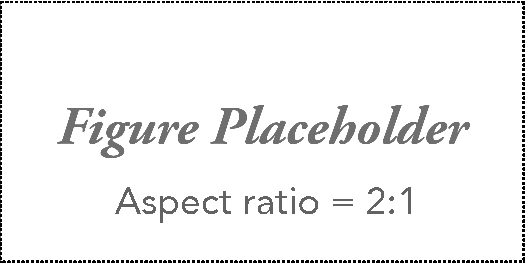
\includegraphics[width=\textwidth]{draft2x1}
		\caption{Top View}
		\label{fig:topview}
	\end{subfigure}
	%
	\begin{subfigure}[b]{0.475\textwidth}
		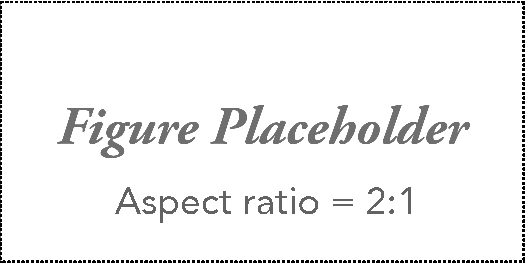
\includegraphics[width=\textwidth]{draft2x1}
		\caption{Side View}
		\label{fig:sideview}
	\end{subfigure}

	\begin{subfigure}[b]{0.475\textwidth}
		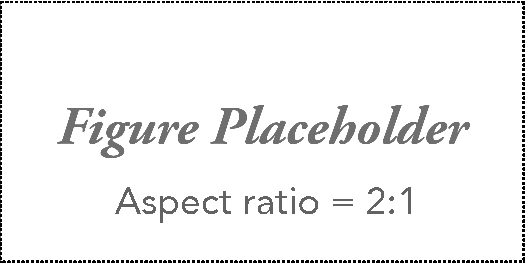
\includegraphics[width=\textwidth]{draft2x1}
		\caption{Front View}
		\label{fig:frontview}
	\end{subfigure}
	%
	\begin{subfigure}[b]{0.475\textwidth}
		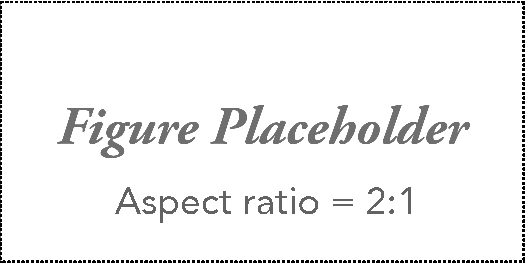
\includegraphics[width=\textwidth]{draft2x1}
		\caption{Rendered View}
		\label{fig:renderedview}
	\end{subfigure}
	\caption{Current drawings and rendering of our conceptual aircraft design.}
	\label{fig:prelimdrawings}
\end{figure}

%Preliminary design / sizing results

After making some decisions about the overall configuration of our aircraft (details on our decision process will be included in the Design Report), we arrived at the configuration seen in \cref{fig:prelimdrawings}.
{\color{BYUred}[COMMENT ON MAJOR FEATURES OF THE CONFIGURATION, GIVE SOME BASIC JUSTIFICATION, LIKE "WE CHOSE THIS BECAUSE IT WOULD WORK WELL FOR THIS REQUIREMENT"]}

Using common hand calculation level formulas, we arrived at a conceptual design with the following specifications: a wing span of {\color{BYUred} [X.X ft]}, aspect ratio of {\color{BYUred} [X.X]}, wing loading of {\color{BYUred} [X.X lbs/ft$^2$]}, horizontal and vertical tail volume ratios of {\color{BYUred} [X.X]} and {\color{BYUred} [X.X]} respectively, stall velocity of {\color{BYUred} [X.X ft/sec]}, and take-off distance of {\color{BYUred} [X.X ft]}.  {\color{BYUred}[INCLUDE ANY OTHER PERTINENT PARAMETERS HERE AS WELL!]}
{\color{BYUred}[DISCUSS ANY INTERESTING FEATURES SPECIFIC TO THIS YEAR'S REQUIREMENTS: ATTACHMENTS, FOLDING THINGS, DEPLOYMENT STUFF, ETC. THAT HAVE BEEN DECIDED IN THE CONCEPTUAL DESIGN.]}
\lipsum[1]

%%%%%%%%%%%%%%%%%%%%%%%%%%%%%%%
%%%% - Sensitivity Study - %%%%
%%%%%%%%%%%%%%%%%%%%%%%%%%%%%%%
\subsection{Sensitivity Study}
\label{ssec:SensitivityStudy}

%Figure related to sensitivity study, move around to get formatting correct...

For our sensitivity study, we first differentiated between design variables that could increase/decrease our score and those that were only related to the minimum constraints. Based on the scoring metrics, we found the parameters that could affect the score to be: wing area, aircraft empty weight (including batteries), total lap distance, number of syringes, number of vial boxes, and available power.  To perform our study, we took our basic parameters and ran them through common hand calculations to find the mission objective scores. In order to normalize the scores as they are in the competition, we ran the analysis first without normalization, from which we saved the maximum scores to simulate the competition normalization. We then used those maxima as the normalization factors and re-ran the analysis.  In our analysis (results shown in \cref{fig:sensitivity}), we found that the wing area and parasitic drag (not plotted) coefficient had the same sensitivities, thus we want to minimize drag and maximize wing loading (while still being able to take off).  The available power was also important, and can be affected by increasing battery capacity, discharge rate, or voltage, or increasing system efficiency. Interestingly, the lap distance is highly sensitive, thus we want to minimize turn radius without tripping the 5g sensors. Obviously the number of payload units carried highly effects the overall score. Note that the number of payload units, which are non-continuous in reality, both result in stepped outputs, but the resolution of the number of syringes is fine enough that it looks continuous in \cref{fig:sensitivity}). We should also note that the aircraft empty weight had a relatively negligible effect on the overall sensitivity, but is important to keep in mind when designing for a feasible aircraft.